\def\year{2020}\relax
%File: formatting-instruction.tex
\documentclass[letterpaper]{article} % DO NOT CHANGE THIS
\usepackage{aaai20}  % DO NOT CHANGE THIS
\usepackage{times}  % DO NOT CHANGE THIS
\usepackage{helvet} % DO NOT CHANGE THIS
\usepackage{courier}  % DO NOT CHANGE THIS
\usepackage[hyphens]{url}  % DO NOT CHANGE THIS
\usepackage{graphicx} % DO NOT CHANGE THIS
\urlstyle{rm} % DO NOT CHANGE THIS
\def\UrlFont{\rm}  % DO NOT CHANGE THIS
\usepackage{graphicx}  % DO NOT CHANGE THIS
\frenchspacing  % DO NOT CHANGE THIS
\setlength{\pdfpagewidth}{8.5in}  % DO NOT CHANGE THIS
\setlength{\pdfpageheight}{11in}  % DO NOT CHANGE THIS


% new packages used by us
\usepackage{epsfig}
\usepackage{amsmath}
\DeclareMathOperator{\sign}{sign}

\usepackage{amssymb}
\usepackage{bbm}
\usepackage{booktabs, multirow}

%\usepackage{natbib}
\usepackage{xcolor}

\usepackage{paralist}
%\usepackage[font=small]{caption}

%\graphicspath{{figures/}}


%\newcommand{\NOTE}[1]{\textcolor{red}{[NOTE: #1]}}
\newcommand{\NOTE}[1]{\textcolor{black}{}}
\newcommand{\abc}[1]{\textcolor{black}{#1}}

\newcommand{\zq}[1]{\textcolor{black}{#1}} % Modifications
%\newcommand{\ZQ}[1]{\textcolor{blue}{[ZQ: #1]}} % ZQ's notes
\newcommand{\ZQ}[1]{\textcolor{black}{}} % ZQ's notes

\newcommand{\abcn}[1]{\textcolor{black}{#1}}
\newcommand{\CUT}[1]{}

\newcommand{\citet}[1]{\citeauthor{#1}\shortcite{#1}}
\newcommand{\citep}{\cite}
\newcommand{\citealp}[1]{\citeauthor{#1} \citeyear{#1}}


% \nocopyright
%PDF Info Is REQUIRED.
% For /Author, add all authors within the parentheses, separated by commas. No accents or commands.
% For /Title, add Title in Mixed Case. No accents or commands. Retain the parentheses.

%Leave this
% /Title ()
% Put your actual complete title (no codes, scripts, shortcuts, or LaTeX commands) within the parentheses in mixed case
% Leave the space between \Title and the beginning parenthesis alone
% /Author ()
% Put your actual complete list of authors (no codes, scripts, shortcuts, or LaTeX commands) within the parentheses in mixed case.
% Each author should be only by a comma. If the name contains accents, remove them. If there are any LaTeX commands,
% remove them.

% DISALLOWED PACKAGES
% \usepackage{authblk} -- This package is specifically forbidden
% \usepackage{balance} -- This package is specifically forbidden
% \usepackage{caption} -- This package is specifically forbidden
% \usepackage{color (if used in text)
% \usepackage{CJK} -- This package is specifically forbidden
% \usepackage{float} -- This package is specifically forbidden
% \usepackage{flushend} -- This package is specifically forbidden
% \usepackage{fontenc} -- This package is specifically forbidden
% \usepackage{fullpage} -- This package is specifically forbidden
% \usepackage{geometry} -- This package is specifically forbidden
% \usepackage{grffile} -- This package is specifically forbidden
% \usepackage{hyperref} -- This package is specifically forbidden
% \usepackage{navigator} -- This package is specifically forbidden
% (or any other package that embeds links such as navigator or hyperref)
% \indentfirst} -- This package is specifically forbidden
% \layout} -- This package is specifically forbidden
% \multicol} -- This package is specifically forbidden
% \nameref} -- This package is specifically forbidden
% \natbib} -- This package is specifically forbidden -- use the following workaround:
% \usepackage{savetrees} -- This package is specifically forbidden
% \usepackage{setspace} -- This package is specifically forbidden
% \usepackage{stfloats} -- This package is specifically forbidden
% \usepackage{tabu} -- This package is specifically forbidden
% \usepackage{titlesec} -- This package is specifically forbidden
% \usepackage{tocbibind} -- This package is specifically forbidden
% \usepackage{ulem} -- This package is specifically forbidden
% \usepackage{wrapfig} -- This package is specifically forbidden
% DISALLOWED COMMANDS
% \nocopyright -- Your paper will not be published if you use this command
% \addtolength -- This command may not be used
% \balance -- This command may not be used
% \baselinestretch -- Your paper will not be published if you use this command
%  -- No page breaks of any kind may be used for the final version of your paper
% \columnsep -- This command may not be used
%  -- No page breaks of any kind may be used for the final version of your paper
% \pagebreak -- No page breaks of any kind may be used for the final version of your paperr
% \pagestyle -- This command may not be used
% \tiny -- This is not an acceptable font size.
% \vspace{- -- No negative value may be used in proximity of a caption, figure, table, section, subsection, subsubsection, or reference
% \vskip{- -- No negative value may be used to alter spacing above or below a caption, figure, table, section, subsection, subsubsection, or reference


\setcounter{secnumdepth}{2} %May be changed to 1 or 2 if section numbers are desired.

% The file aaai20.sty is the style file for AAAI Press
% proceedings, working notes, and technical reports.
%
\setlength\titlebox{2.5in} % If your paper contains an overfull \vbox too high warning at the beginning of the document, use this
% command to correct it. You may not alter the value below 2.5 in
\title{3D Crowd Counting via Multi-View Fusion with 3D Gaussian Kernels}

% Your title must be in mixed case, not sentence case.
% That means all verbs (including short verbs like be, is, using,and go),
% nouns, adverbs, adjectives should be capitalized, including both words in hyphenated terms, while
% articles, conjunctions, and prepositions are lower case unless they
% directly follow a colon or long dash

%\author{Written by AAAI Press Staff\textsuperscript{\rm 1}\thanks{Primarily Mike Hamilton of the Live Oak Press, LLC, with help from the AAAI Publications Committee}\\ \Large \textbf{AAAI Style Contributions by
%Pater Patel Schneider,} \\ \Large \textbf{Sunil Issar, J. Scott Penberthy, George Ferguson, Hans Guesgen}\\ % All authors must be in the same font size and format. Use \Large and \textbf to achieve this result when breaking a line
%\textsuperscript{\rm 1}Association for the Advancement of Artificial Intelligence\\ %If you have multiple authors and multiple affiliations
%% use superscripts in text and roman font to identify them. For example, Sunil Issar,\textsuperscript{\rm 2} J. Scott Penberthy\textsuperscript{\rm 3} George Ferguson,\textsuperscript{\rm 4} Hans Guesgen\textsuperscript{\rm 5}. Note that the comma should be placed BEFORE the superscript for optimum readability
%2275 East Bayshore Road, Suite 160\\
%Palo Alto, California 94303\\
%publications20@aaai.org % email address must be in roman text type, not monospace or sans serif
%}


\author{Qi Zhang, Antoni B. Chan \\ %\textsuperscript{\rm 1} \\
%\thanks{Primarily Mike Hamilton of the Live Oak Press, LLC, with help from the AAAI Publications Committee}
%\Large \textbf{AAAI Style Contributions by Pater Patel Schneider,} \\
%\Large \textbf{Sunil Issar, J. Scott Penberthy, George Ferguson, Hans Guesgen}\\ % All authors must be in the same font size and format. Use \Large and \textbf to achieve this result when breaking a line
Department of Computer Science, City University of Hong Kong\\ %If you have multiple authors and multiple affiliations
% use superscripts in text and roman font to identify them. For example, Sunil Issar,\textsuperscript{\rm 2} J. Scott Penberthy\textsuperscript{\rm 3} George Ferguson,\textsuperscript{\rm 4} Hans Guesgen\textsuperscript{\rm 5}. Note that the comma should be placed BEFORE the superscript for optimum readability
Tat Chee 83, Kowloon Tong, Hong Kong SAR, China\\
%Palo Alto, California 94303\\
qzhang364-c@my.cityu.edu.hk, abchan@cityu.edu.hk % email address must be in roman text type, not monospace or sans serif
}




 \begin{document}

\maketitle

\begin{abstract}
  Crowd counting has been studied for decades and a lot of works have achieved %quite
  good performance, especially the DNNs-based density map estimation methods. Most existing crowd counting works focus on single-view counting, while few works have studied multi-view counting for large and wide scenes, where multiple cameras are used.
   %However, hand-crafted features and detection-based framework dramatically limit the previous multi-view counting methods' performance.
  Recently, an end-to-end multi-view crowd counting method called multi-view multi-scale (MVMS) has been proposed, which fuses multiple camera views using a CNN to predict a 2D scene-level density map on the ground-plane. Unlike MVMS, we propose to solve the multi-view crowd counting task through 3D feature fusion with 3D scene-level density maps, instead of the 2D ground-plane ones. %Gaussian kernels as ground-truth instead of the 2D ones.
  Compared to 2D fusion, the 3D fusion extracts more information of the people along $z$-dimension (height), which helps to solve the scale variations across multiple views. The 3D density maps still preserve the 2D density maps property that the sum is the count, while also providing 3D information about the crowd density.
   %' ``sum=counting number'' property as well as provides a more vivid representation for the crowd flow. Besides,
  We also explore the projection consistency among the 3D prediction and the ground-truth in the 2D views
  %is explored to
  to further enhance the counting performance. The proposed method is tested on 3 multi-view counting datasets and achieves better or comparable counting performance to the state-of-the-art.
\end{abstract}
\section{Introduction}

\begin{figure}[t]
\centering
   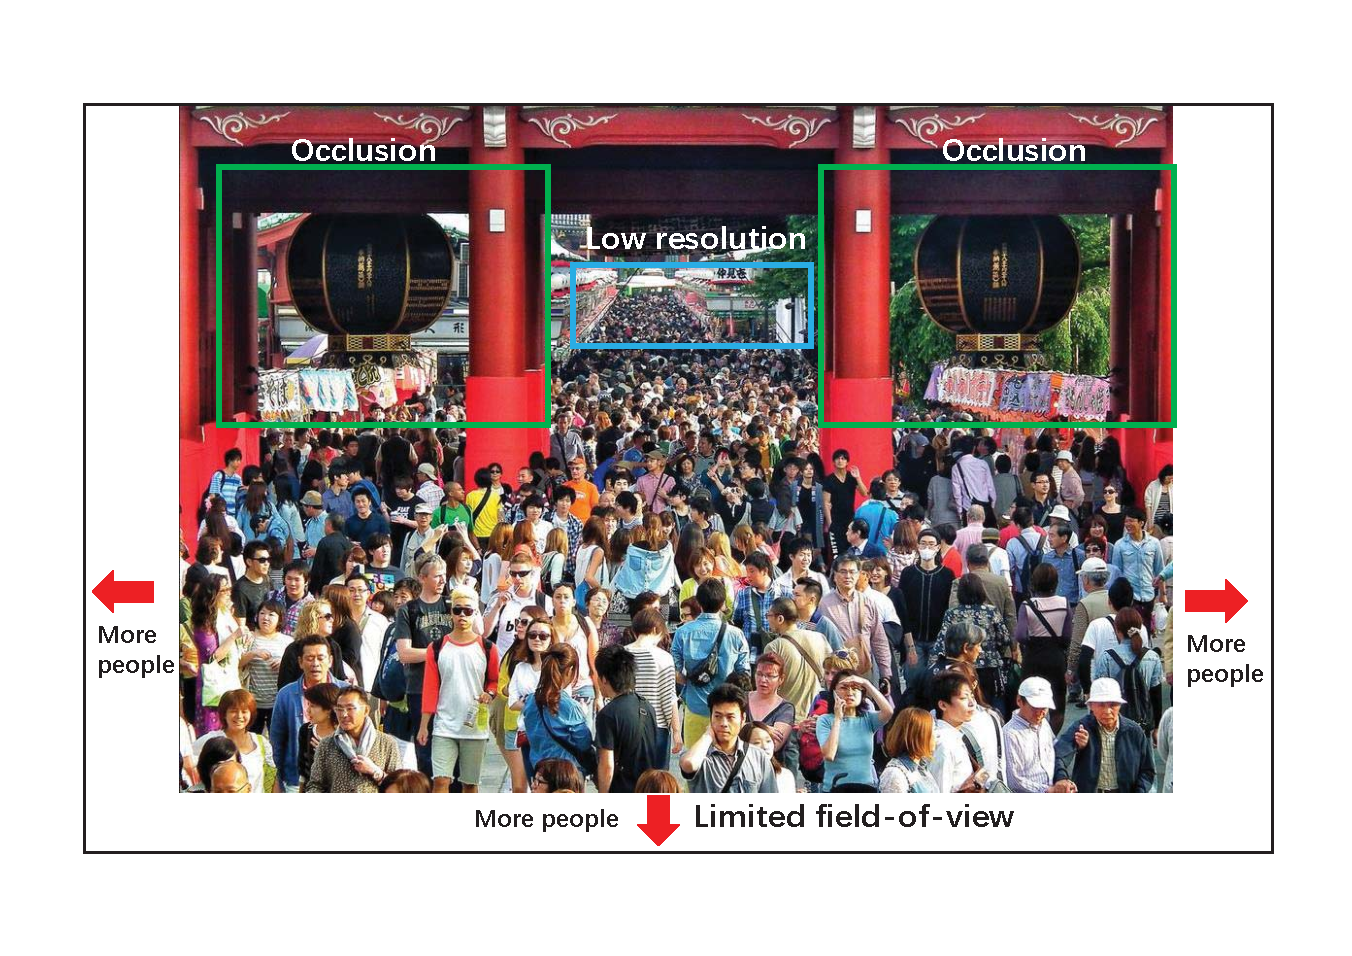
\includegraphics[width=0.95\columnwidth]{Fig_3examples.pdf}
   \caption{An example for the limitation of single-view counting for large and wide scenes: limited field-of-view, low resolution and severe occlusion. This image is from the ShanghaiTech dataset \citep{zhang2015cross}.
   %More similar examples in the current counting datasets can be found in the Supplemental.
   }
\label{fig:example}
\end{figure}

\begin{figure*}[t]
\centering
   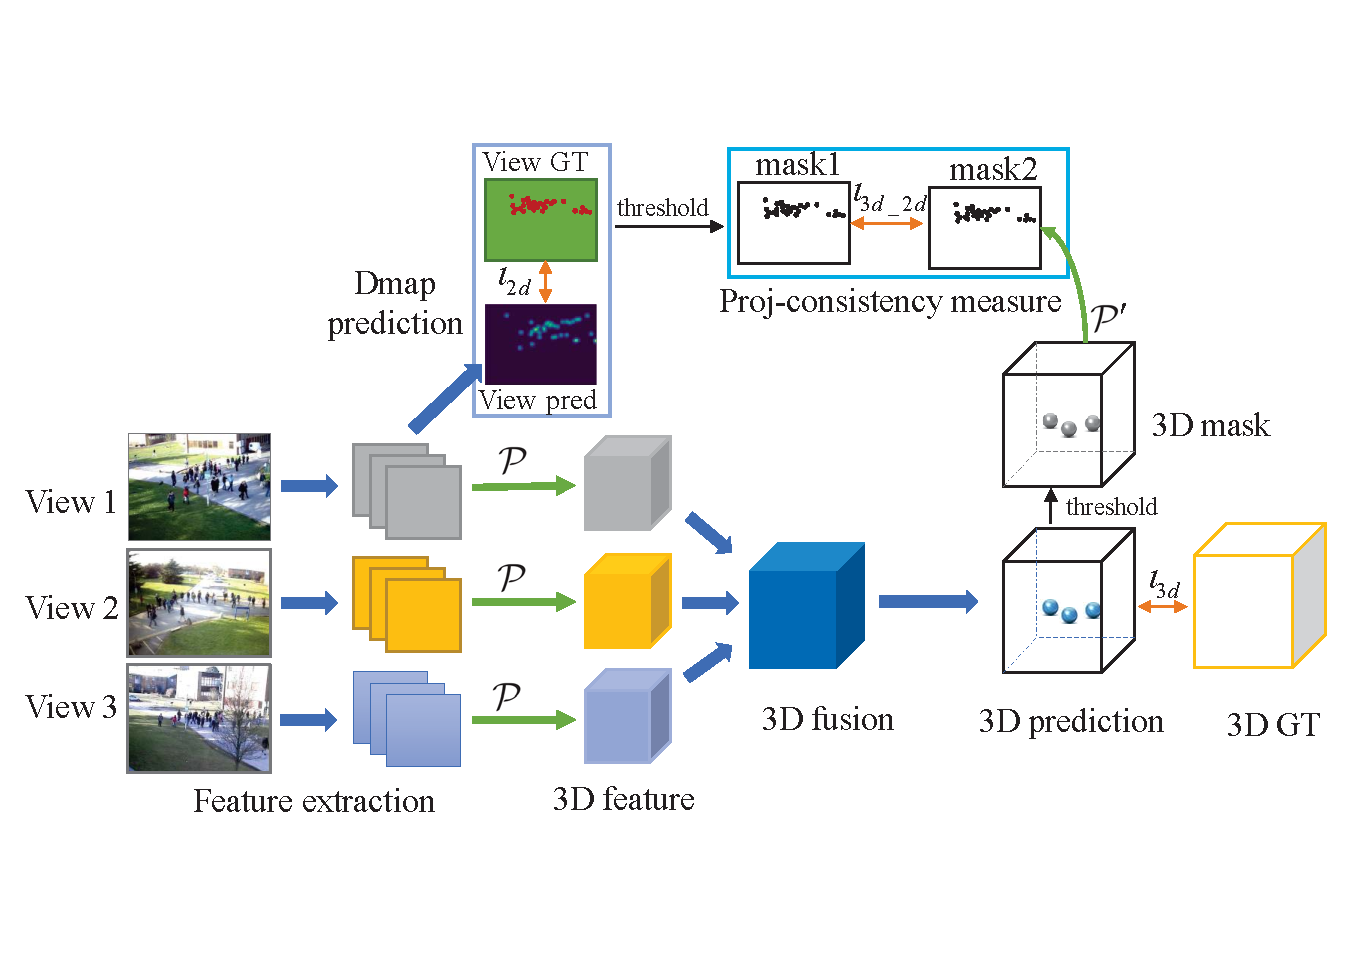
\includegraphics[width=0.7\textwidth]{Fig_pipeline.pdf}
   \caption{The pipeline of 3D crowd counting. Single-view features are extracted and then projected to the 3D world on multiple height planes. The projected 3D features are concatenated and fused to output the 3D density map prediction (loss $l_{3d}$). Each camera-view prediction branch decode the 2D features to obtain the 2D camera-view predictions (loss $l_{2d}$). Finally, the 3D prediction is back-projected to each camera-view, and the the projection consistency between the camera-view ground-truth and the back-projected prediction %3D-to-2D predictions
   is measured (loss $l_{3d\_2d}$).}
\label{fig:pipeline}
\end{figure*}

Single-view crowd counting has been studied for decades and has achieved promising performance on the existing counting datasets \citep{zhang2015cross,Idrees2013Multi,zhang2016single,Chan2008Privacy,Chen2012Feature,idrees2018composition}. However, in real-world applications, there are several situations where single-view counting cannot perform well (e.g., see Fig.~\ref{fig:example}): 1) The scene is too wide (such as a park or a football match stadium) where a single camera's field-of-view is limited and cannot cover the whole scene; 2) The scene is too long (such as the underground train platform) where the people who are far away from the camera have very low resolution and the counting methods' performance drops on these people; 3) The scene contains a lot of obstacles, such as vehicles, building structures or \emph{etc.}, where many people are heavily or totally occluded. Under the 3 conditions, the current single-view counting methods are inaccurate, because many people are miscounted due to limited field-of-view, low resolution and severe occlusion.

To address the aforementioned situations, multiple cameras should be deployed, and the multi-view information should be fused to enhance the counting performance for complicated scenes. A few works \citep{li2012people,Ryan2014Scene,Tang2014Cross,Ge2010Crowd} have considered multi-view counting. However, the hand-crafted features and the foreground extraction steps limit their performance. % a lot.
Recently, a CNN-based multi-view counting method \citep{zhang2019wide} was proposed, which improved the counting performance on wide-area scenes.
% \cite{ferryman2009pets2009, ristani2016MTMC, zhang2019wide}.
In their paper, the multi-view information (camera-view density maps or feature maps) are projected to the same 2D plane in the 3D scene (at the height of a person), and then fused to predict the 2D scene-level density maps on the ground-plane. Several fusion methods are considered, including late and early fusion, and a multi-view multi-scale early fusion model (MVMS), which handles both the inter- and intra-view scale variations.

The disadvantage of the 2D-to-2D projection in \citep{zhang2019wide} is that the features of the same person from different views may not line up correctly due to the approximation that all features come from the same height in the 3D world. Clearly this is not true for features extracted from the heads and feet of the people.
To address this problem,
in this paper,
we propose to use 3D projection and 3D feature fusion to perform the multi-view counting task. Our proposed method consists of following components (see Fig.~\ref{fig:pipeline}): 1) \emph{Single view feature extraction and density map prediction}: 2D single-view features are extracted and then decoded to the 2D density map predictions; 2) \emph{2D-to-3D projection}: A differentiable projection layer together with the camera parameters are used to perform the fixed 3D projection from image plane to 3D world; 3) \emph{3D fusion and prediction}: The projected multi-view 3D features are fused using 3D CNN layers to predict the 3D scene-level density map \CUT{and $z$-dim full-size 3D filters are adopted to handle the scale variation issue}; 4) \emph{Projection consistency between the 3D prediction and 2D views}: The 3D prediction is back-projected to each camera view and a loss between the camera view prediction and back-projected 3D prediction is added to enhance the multi-view counting performance.

%\NOTE{maybe this is not true, since the difference in feature scale is caused by different distances to each camera.}
In our approach, the 3D projection provides more information of the people, and the projected people's scales along the $z$-dimension in the 3D world are similar to each other (decided by the people height), which suggests the scale variation issue among multiple views can be tackled without the scale-selection module like in MVMS. In addition, a 3D density map with 3D Gaussian kernels is used to represent the crowd in the scene, instead of the 2D scene-level density maps. The 3D density map can provide more information about the crowd in 3D, e.g., the elevation of the crowd. % vivid representation of the crowd.
\CUT{The prediction of the 3D density map is also used as an %And the 3D prediction can be used an
intermediate representation to enforce the projection consistency across the camera views, which can further improve the multi-view counting performance.
%Besides, except the scene-level 3D ground-truth, 3D ground-truth based on one or partial views are also added, which forms a stage-by-stage supervision fashion.
}

In summary, the main contributions of our paper are:
%\begin{itemize}
\begin{compactitem}
%\setlength\itemsep{0em}
  \item We propose an end-to-end DNNs-based 3D multi-view counting method that predicts 3D density maps, which provides information about the crowd in 3D. To the best of our knowledge, this is the first study of 3D scene-level multi-view crowd counting.
          %The 3D Gaussian kernels are used instead of 2D ones, which can provide a more vivid representation of the crowd as well as indicate the crowd count.
  \item \zq{Unlike the previous methods, we use 3D projection and 3D fusion, which can help to deal with the scale variation issue without the scale selection module}.
      %\NOTE{maybe...} \zq{[Do need better experiment results to prove it.]}
  \item The projection consistency between the camera-view ground-truth and the back-projected 3D predictions is explored to further boost the multi-view counting performance. The proposed method can achieve better or comparable counting performance to the state-of-art.
      %projected 3D-to-2D predictions
\end{compactitem}
%\end{itemize}


%-------------------------------------------------------------------------
\section{Related Work}
In this section, we will review the existing single-view and multi-view counting methods. We also review 3D object reconstruction using deep neural networks (DNNs).

\subsection{Single-view counting}
Single-view crowd counting has achieved satisfactory performance on the existing counting datasets, especially the DNN-based density map estimation methods. \citealp{zhang2015cross} proposed a single-column CNN framework to directly estimate the density maps from the images. Scale variations due to perspective changes %and distance differences
 is a critical issue in the crowd counting task, which can limit the performance, and many %. Therefore, many
 methods have been proposed to handle scale variations \citep{boominathan2016crowdnet,zhang2016single,sam2017switching,Kang2018Crowd,onoro2016towards}.
% and improve the counting performance.
% First, the multi-column architectures were adopted to model people of different scales, such as Crowdnet \citep{boominathan2016crowdnet}, MCNN \citep{zhang2016single} and Switch-CNN \citep{sam2017switching}. Alternatively, the image pyramid was fed into the multi-column network to achieve the scale consistency among the scale-variant crowd \citep{Kang2018Crowd,onoro2016towards}.
 \citealp{sindagi2017generating} proposed the contextual pyramid CNN (CP-CNN) to incorporate global and local context information in the crowd counting framework. Furthermore, extra information and more sophisticated networks were utilized to further improve the counting performance \citep{idrees2018composition,Wang2019Learning,ranjan2018iterative,cao2018scale,li2018csrnet,liu2018decidenet,shen2018crowd,Jiang2019Crowd,Liu2019Context}.
 \citealp{kang2017incorporating} proposed an adaptive convolution neural network (ACNN) by utilizing the context (camera height and angle) as side information in the counting framework.
 \citealp{shi2019revisiting} integrated the perspective information to provide additional knowledge of the person scale change in an image.
 \citealp{Lian2019Density} proposed a regression guided detection network (RDNet) for RGB-D crowd counting.
 %\cite{li2018csrnet} replaced pooling operations in the CNN layers with dilated kernels to deliver larger reception fields and achieved better counting performance.
 \citealp{Liu2019Recurrent} proposed Recurrent Attentive Zooming Network to zoom high density regions for higher-precision counting and localization.

The single-view based counting methods cannot handle the situations when the camera cannot cover the whole scene,  the occlusions in the scene are too severe, or the people are in low resolution due to long distance to the camera. Therefore, multiple cameras should be adopted to improve the counting performance for these wide-area scenes.

\subsection{Multi-view counting}

%In addition to single-view counting, a few works have studied multi-view counting.
Traditional multi-view counting methods can be divided into 3 categories: detection/tracking based \citep{dittrich2017people,li2012people,ma2012reliable,Maddalena2014people}, regression based \citep{Ryan2014Scene,Tang2014Cross}, 3D cylinder based \citep{Ge2010Crowd}. These multi-view counting methods have several limitations. First, they need to utilize foreground extraction techniques to segment the crowd from background. Therefore, the effectiveness of the foreground extraction step limits the final counting performance. Second, hand-crafted features are used both in the people detection or crowd count regression. The hand-crafted features lack representation ability, which reduces the robustness and the performance of the methods. Third, these methods are mainly performed and tested on the PETS2009 \citep{ferryman2009pets2009}, which is a multi-view dataset with small crowd numbers and staged crowd behavior.

Recently, \citealp{zhang2019wide} proposed a DNN-based multi-view counting method MVMS and a new larger multi-view counting dataset CityStreet. MVMS first extracts camera-view information (density maps or features), and then projects them to the average-height plane in the 3D scene with the given camera parameters. Next, the projected features are fused and decoded to predict the scene-level density maps (on the average height plane). Our proposed method differs from MVMS in the several aspects: 1) instead of using average-height projection, we use multi-height projection, which \abc{spatially aligns the person's features (e.g., head, body and feet features) in 3D, making it easier to} find the geometric correspondence across views (See Fig. \ref{fig:3dprojection}); 2) we predict a 3D crowd density map, generated using 3D Gaussian kernels, which provides distribution of the crowd in 3D space; 3) the 3D density map prediction is back-projected to each camera view, and compared with the 2D ground-truth density map of the camera view, which defines a projection consistency loss for improving the accuracy.


\subsection{DNN-based 3D reconstruction}

%Recently,
%DNN-based 3D object reconstruction has become a popular research topic.
Our 3D crowd counting method is related to a few works on DNN-based 3D object reconstruction and human pose estimation. \citealp{yan2016perspective} proposed an unsupervised single-view 3D object reconstruction method utilizing the projection loss defined by the perspective transformation.
%\citealp{choy20163d} proposed a 3D recurrent neural network architecture for multi-view 3D object reconstruction in which the output reconstruction is gradually refined step-by-step.
\citealp{choy20163d} proposed a 3D RNNs architecture to gradually refine the multi-view 3D object reconstruction step-by-step.
%\citealp{kar2017learning} proposed an end-to-end 3D reconstruction method, which leverages the 3D geometry constraint of features through projection and unprojection operations.
\citealp{kar2017learning} leveraged the 3D geometry constraint of features through projection and unprojection operations in the 3D reconstruction method.
%\citealp{lin2018learning} proposed to use 2D convolution to predict the point cloud of an object from multi-view points, improving the efficiency compared to 3D convolutions.
\citealp{huang2018deepmvs} presented DeepMVS to %method, which
 produce a set of plane-sweep volumes and then predict high-quality disparity maps.
\citealp{Iskakov2019Learnable} proposed two learnable triangulation methods for 3D human pose estimation: algebraic triangulation and volumetric aggregation.

\par
It can be observed that the existing DNNs-based 3D reconstruction methods are mainly focused on the reconstruction of a single object (see datasets ShapeNet \citep{chang2015shapenet} and IKEA \citep{lpt2013ikea}, or human pose). Our proposed method can also be regarded as predicting a 3D representation from multiple viewpoints, but differs from the existing DNN-based 3D object reconstruction in several aspects. First, the proposed method can do more than \zq{3D shape reconstruction}, because the 3D Gaussian kernels can represent the crowd's 3D distribution as well as indicate the crowd count. Second, unlike the previous 3D object reconstruction, the proposed method targets at the scene-level representation (all people in the scene), not only a single object. Furthermore, we exploit the relationship between the 2D camera-view density maps and 3D scene-level density maps to obtain a projection consistency loss.



\section{3D Counting via 3D Projection and Fusion}

We follow the setup of multi-view counting in \citealp{zhang2019wide}: we assume fixed cameras with known intrinsic and extrinsic camera parameters, and synchronized camera frames across views. In contrast to \citealp{zhang2019wide}, which is based on 2D ground-plane density maps, we generate 3D ground-truth density maps %is obtained
by convolving the 3D ground-truth annotations with fixed-width 3D Gaussian kernels. The 3D ground-truth annotation coordinates are calculated from the 2D view annotations and people correspondence across views (see Section 4 for more details).

In this section, we introduce the end-to-end DNNs-based 3D crowd counting method %based on multiple views
consisting of following stages. 1) \emph{Single view feature extraction and density map prediction}: 2D single-view features are extracted and  decoded to predict a 2D camera-view density map; 2) \emph{2D-to-3D projection}: a differentiable projection layer using the camera parameters projects the camera-view feature maps from the image plane to multiple height-planes in the 3D world; 3) \emph{3D fusion and prediction}: the projected multi-view 3D features are fused to predict the 3D density maps using 3D CNN layers; 4) \emph{Projection consistency between the 3D prediction and 2D views}: the 3D prediction is back-projected to each camera view, %transformed to each single views
and then compared with the corresponding camera-view 2D ground-truth using loss to refine the 3D prediction.



% ### A TABLE showing the layer setting ######
\begin{table}[t]
\centering
\begin{tabular}{ll}
\scriptsize
\begin{tabular}{|c|c|}
\hline
\multicolumn{2}{|c|}{Single-view branch} \\ \hline
Layer         & Filter      \\ \hline
\multicolumn{2}{|c|}{Feature extraction} \\ \hline
conv 1             & $16\! \times\! 1\! \times\!  5\!  \times\!  5$     \\ %\hline
conv 2             & $16\!  \times\!  16\!  \times\!  5\!  \times\!  5$    \\ %\hline
pooling   & $2\!  \times\!  2\!  $         \\ %\hline
conv 3             & $32\!  \times\!  16\!  \times\!  5\!  \times\!  5$   \\ %\hline
conv 4             & $32\!  \times\!  32\!  \times\!  5\!  \times\!  5$ \\ %\hline
pooling   & $2\!  \times\!  2\!  $          \\ \hline

\multicolumn{2}{|c|}{Density map prediction} \\ \hline

conv 5             & $64\!  \times\!  32\!  \times\!  5\!  \times\!  5$ \\ %\hline
conv 6             & $32\!  \times\!  64\!  \times\!  5\!  \times\!  5$ \\ %\hline
conv 7             & $1\!  \times\!  32\!  \times\!  5\!  \times\!  5$  \\ \hline
\end{tabular}
&
\scriptsize
\begin{tabular}{|c|c|}
\hline
\multicolumn{2}{|c|}{3D Fusion module}  \\ \hline
Layer & Filter     \\ \hline
   concatenation   &  - \\ %\hline
3D conv 1     & $32\!  \times\!  n\!   \times\!  5\!  \times\!  5\!  \times\!7$   \\ %\hline
3D conv 2     & $64\!  \times\!  32\!  \times\!  5\!  \times\!  5\!  \times\!7$  \\% \hline
3D conv 3     & $128\! \times\!  64\!  \times\!  5\!  \times\!  5\!  \times\!7$ \\
3D conv 4     & $64\!  \times\!  128\! \times\!  5\!  \times\!  5\!  \times\!7$ \\
3D conv 5     & $32\!  \times\!  64\!  \times\!  5\!  \times\!  5\!  \times\!7$ \\
3D conv 6     & $32\!  \times\!  32\!  \times\!  5\!  \times\!  5\!  \times\!7$ \\
3D conv 7     & $1\!   \times\!  32\!  \times\!  5\!  \times\!  5\!  \times\!7$ \\

\hline
\end{tabular}
\end{tabular}
%%removedVspace
\caption {The layer settings for the camera-view feature extraction and density map prediction branches (left), and the 3D fusion module (right). %Two max-pooling layers are used in FCN-7.
The filter dimensions are output channels, input channels, and filter size $w_0\!  \times\!  h_0\!  \times\!d_0$ ($d_0=1$ in 2D conv layers). }
\label{table:layer_setting}
%%removedVspace
\end{table}

\subsection{Single-view branch}
\par
Each camera-view image is fed into a CNN  to extract the camera-view features. The 2D camera-view features are decoded by another CNN to predict the camera-view density maps. The camera-view feature extraction and density map prediction layer settings can be found in Table \ref{table:layer_setting} left.


\par
Here, the camera-view prediction branches contribute to the model performance in 2 aspects. First, the camera-view prediction branches together with the 2D density map supervision  improves the training of the camera-view feature extraction. A similar strategy is used in \citealp{zhang2019wide}, where the camera-view prediction branches are used in the first stage for pre-training. Second, the camera-view prediction branches force the 2D feature representation to be consistent with the 3D feature representation, and the difference between them is the geometric projection. %. And the only difference between them is just a fixed geometry projection operation.
This constraint is natural because the 2D and 3D observations are linked by the geometry projection, and the same link still exists between the 2D and 3D feature representations. The 2D-3D feature representation constraint was also used in \citealp{girdhar2016learning}, where the 3D representation is forced to be able to predict the 2D observations from it. Furthermore, this constraint can improve the final 3D prediction performance (see ablation study for more details).

\par \zq{Suppose} there are $N$ camera-views, the density map prediction for the $i_{th}$ view is $V_i\in {R^{h \times w}} $ and the corresponding ground-truth is $V_i^t \in {R^{h \times w}}$, then the camera-view density map prediction loss $l_{2d}$ is the mean-square error (MSE):
\begin{align}
  l_{2d} = \frac{1}{wh}\sum_{i=1}^N \parallel V_i - V_i^t \parallel _2^2.
\end{align}


\subsection{2D-to-3D projection}


\begin{figure}[t]
\centering
   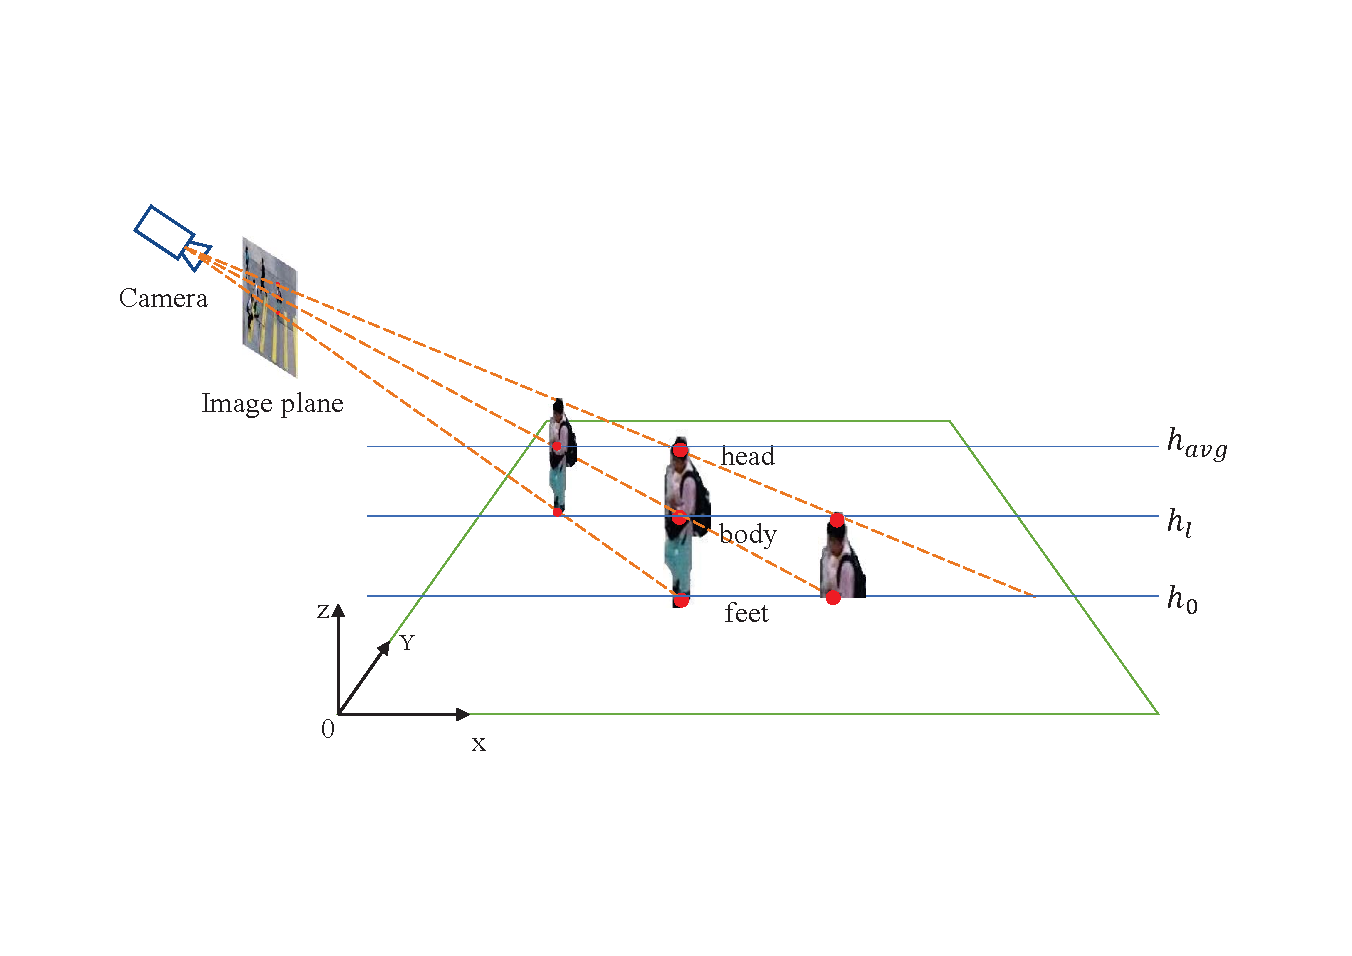
\includegraphics[width=0.95\columnwidth]{Fig_3dprojection.pdf}
   \caption{
   The multi-height projection can extract feature of the people body along $z$ dimension and form a 3D feature representation for the people, which is consistent with the 3D scene. }
\label{fig:3dprojection}
\end{figure}



\par
The extracted camera-view features are projected to the 3D world with a fixed 2D-to-3D projection layer. We assume that the camera intrinsic and extrinsic parameters are both known, which are used to perform the projection. Since each image pixel's corresponding height in the 3D world is unknown, a height range $H$
%\zq{(say $H = \{0, 400, 800, ... , 2400 mm\}$)}
is used in the projection, where each pixel is projected to the 3D world multiple times onto different height planes. Then, the projected features from all height are concatenated along the $z$-dimension %in terms of height
to form a 3D feature representation.
The 2D-to-3D projection layer can be implemented using the Sampler from the Spatial Transformer Networks \citep{Jaderberg2015Spatial} with the known camera calibration parameters (intrinsic and extrinsic).
Suppose that $\cal P$ is the 2D-to-3D projection, $F_i$ stands for the 2D feature presentation of view $i$, and the height range $H = \{h_0, h_1, ..., h_r\}$, then the projected 3D feature representation $(F_{3d})_i$ for view $i$ is
\begin{align}
%  (F_{3d})_i & = {{\cal P}_i} (F_i, H) \\
%             & = [{{\cal P}_i} (F_i, h_0), {{\cal P}_i} (F_i, h_1), ..., {{\cal P}_i} (F_i, h_r)] ,
  (F_{3d})_i = {{\cal P}_i} (F_i, H)
             = [{{\cal P}_i} (F_i, h_0), ..., {{\cal P}_i} (F_i, h_r)] ,
\end{align}
where $[\cdot]$ is concatenation %operation
along the $z$-dimension (height).

\par
In \citealp{zhang2019wide}, the fixed-height projection was used where all pixels were projected to the average height (1750mm). Compared to average-height projection, the multi-height projection can output a body feature representation along $z$-dim (e.g., head, body and feet features, see Fig. \ref{fig:3dprojection}), which allows the network to better identify the location of the person through the 3D alignment of the features.


\subsection{3D density map prediction}
After the 2D-to-3D projection, the projected 3D features from multiple views are concatenated (along the feature channel) and then decoded by several 3D convolution layers.
The architecture for the 3D feature decoder layers can be found in Table \ref{table:layer_setting} right.
%\NOTE{add table for settings}
%\ZQ{Done.}
Suppose the 3D prediction is $G \in {R^{a \times b \times d}} $ and the corresponding ground-truth is $G^t \in {R^{a \times b \times d}}$, the 3D prediction loss $l_{3d}$ is the MSE
\begin{align}
  l_{3d} = \frac{1}{abd} \parallel G - G^t \parallel _2^2.
\end{align}





\subsection{3D-to-2D projection consistency measure}
\par
Considering the geometry constraint between 2D observations and the 3D observation, we also require the 3D prediction be consistent with the 2D single view density maps in terms of projection geometry. To achieve this, the 3D prediction $G$ is projected to each camera-view $i$ with a 3D-to-2D projection operation ${\cal P}^{'}$. The projection consistency between the projected 2D density maps and the 2D density map ground-truth is measured and used as part of the loss to further enhance the 3D counting performance.

% ### adding a figure: explain consistency measure ######
\begin{figure}[t]
\centering
   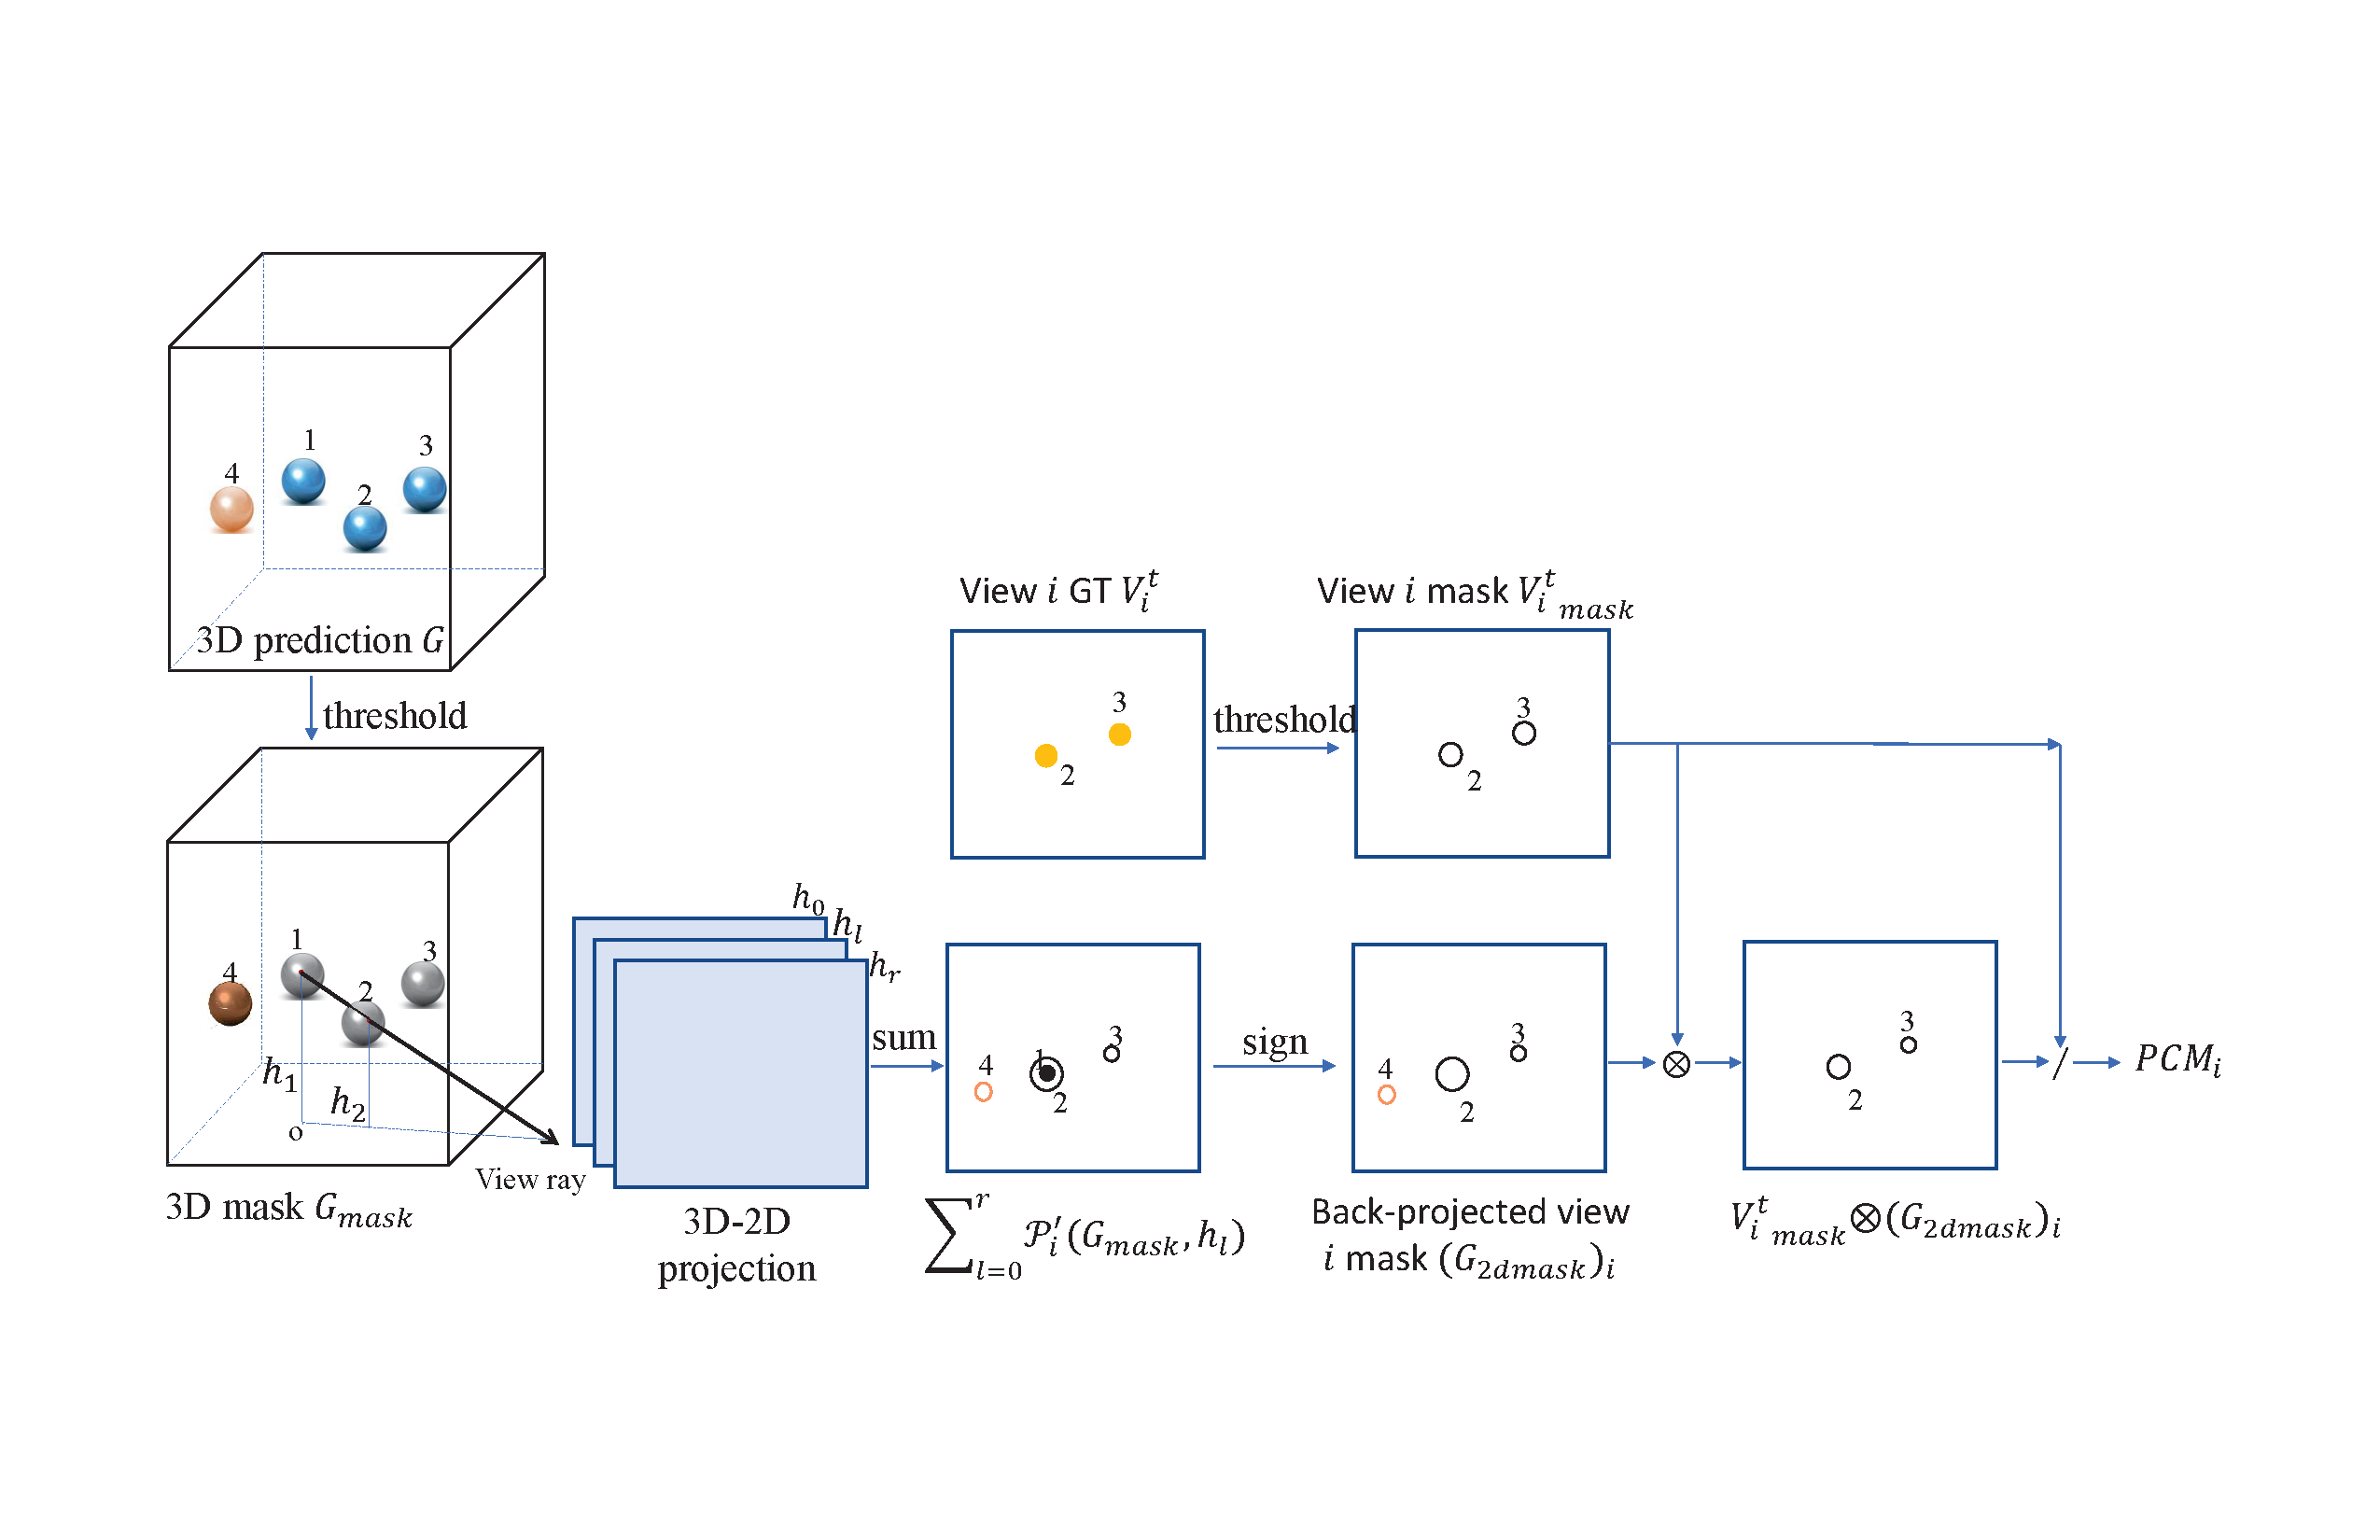
\includegraphics[width=0.95\columnwidth]{Fig_pcm.pdf}
   \caption{Example of projection consistency measure (PCM). \zq{There are 4 people in the 3D prediction, while only Person 2 and Person 3 are visible in the 2D view $i$. Since Person 1 is occluded by Person 2 and Person 4 is totally occluded in view $i$, they are masked out in the PCM calculation.} When the people location in the 3D prediction is not consistent with the 2D ground-truth, the $PCM$ value is low.
%   \NOTE{the figure is a little unclear. try to show the 3d density and 2d GT parts better (use english labels, and the variable names)}
%   \ZQ{Done.}
   }
%%removedVspace
\label{fig:pcm}
\end{figure}


%\subsubsection{3D-to-2D projection}
\textbf{3D-to-2D projection.}~Suppose the $\cal P^{'}$ is the 3D-to-2D projection, $G_{mask}$ is a 3D binary mask which is the 3D prediction $G$ thresholded at $T=10^{-4}$. When performing the projection, each pixel's height of the 2D view plane is also unknown (each 2D image point is corresponding to many 3D points along the view ray without the height information). Therefore, the height range $H = \{h_0, h_1, ..., h_r\}$ is also used in the 3D-to-2D projection. Then the projected 2D mask $(G_{2dmask})_{i}$ for view $i$ can be denoted as,
\begin{align}
      %(G_{2dmask})_{i}  = (\sum^r_{l=0}{\cal P}^{'}_i (G_{mask}, h_l))\cap \mathbbm{1},
      \zq{(G_{2dmask})_{i}  = \sign(\sum^r_{l=0}{\cal P}^{'}_i (G_{mask}, h_l)),}
  %, = {\cal P}^{'}_i(G_{mask}, H) {\cal P}^{'}_i (G_{mask}, h_1), ..., {\cal P}^{'}_i (G_{mask}, h_r) ,
\end{align}
where $\sum$ is summation along the $z$-dimension (height dimension). In the 3D-to-2D projection, the projected 2D pixel value can be regarded as the binary summation along the view ray in the 3D prediction grid (see Fig. \ref{fig:pcm}).

%\subsubsection{Projection consistency measure}
\textbf{Projection consistency measure.}~The main challenge to measure the consistency between the 3D density map prediction and the 2D camera-view density map is that some people who are occluded in a 2D camera-view will be present in the 3D prediction (because they are visible from other views).  Thus the MSE loss cannot be used directly here.
Instead, we measure the consistency between the binary masks produced by thresholding %from
the 3D prediction and the corresponding  2D ground-truth density map, while accounting for inconsistencies due to occlusions (see Fig.~\ref{fig:pcm}).
%Both binary masks are produced by comparing the 3D prediction or the 2D density map ground-truth with a small threshold.
% The reason is that the 3D-to-2D projection operation preserves the people location information rather than the whole people count due to occlusions.

\par
We define the 3D-to-2D projection consistency measure (PCM) for view $i$:
\begin{align}
  PCM_{i} = \frac{\parallel {V_i^t}_{mask} \otimes (G_{2dmask})_{i} \parallel_1}{\parallel {V_i^t}_{mask} \parallel_1 + \alpha},
\end{align}
where $\otimes$ denotes element-wise multiplication, ${V_i^t}_{mask}$ is a binary mask which is the ground-truth density map of view $i$ thresholded at 1e-3, $(G_{2dmask})_{i}$ is the back-projected 3D prediction mask, and $\alpha$=1e-5 is a constant to prevent divide-by-zero.
% in case of zero denominator.
%
The important property of the PCM is that no penalty occurs when an extra person is present in the 3D prediction ($(G_{2dmask})_{i}$), but not the 2D camera-view (e.g., due to occlusion). On the other hand, the PCM will be reduced when a person in the 2D camera-view is missing in the 3D prediction. Finally, the projection consistency loss is defined by summing over the camera-views:
\begin{align}
  l_{3d\_2d} = \sum_{i=1}^{N}(1 - PCM_{i}).
\end{align}

\subsection{Training loss}

Combining all the aforementioned losses, the final loss is
\begin{align}
  l_{all} = l_{3d} + \beta l_{2d} + \gamma l_{3d\_2d}, \label{loss_all}
\end{align}
where $\beta$ and $\gamma$ are hyperparameters for weighting the contributions of each term.
%'s values and the training methods can be found in the Table \ref{table:training_settings} of Experiments and Evaluation section.



\section{Experiments and Evaluation}
In this section, we will discuss the implementation details, and conduct experiments of our proposed 3D crowd counting framework on three multi-view counting datasets.


\begin{table*}
\small
\centering
\begin{tabular}{l|c|c|c}
\hline
    Dataset        & PETS2009      &DukeMTMC    &CityStreet   \\
\hline
    Dmap weighted  & 8.32                                      & 2.12                             & 9.36   \\
    Detection+ReID & 9.41                                       & 2.20                             & 27.60   \\
\hline
    Late fusion \citep{zhang2019wide}         & 3.92             & 1.27                             & 8.12    \\
    Na\"ive early fusion \citep{zhang2019wide} & 5.43             & 1.25                             & 8.10   \\
    MVMS \citep{zhang2019wide}                  &3.49              &\textbf{1.03}                     & 8.01   \\
\hline
    3D counting (ours)                        &\textbf{3.15}        &1.37                           & \textbf{7.54} \\
\hline
\end{tabular}
%%removedVspace
\caption{Experiment results: mean absolute error (MAE) on three multi-view counting datasets. ``3D counting'' uses both single-view branches and the projection consistency measure loss.}
\label{table:results}
\end{table*}




%%%%%%%%%%%%%%%%%%%%%%%%%% ablation study: large table %%%%%

\begin{table*}
\centering
\small
\begin{tabular}{l|ccc@{\hspace{0.1cm}}c|ccc@{\hspace{0.1cm}}c|ccc@{\hspace{0.1cm}}c}
\hline
    Dataset & \multicolumn{4}{c|}{PETS2009}   & \multicolumn{4}{c|}{DukeMTMC}    & \multicolumn{4}{c}{CityStreet}\\
\hline
    $n*h$  & 3D     &3D+2D    & \multicolumn{2}{c|}{3D+2D+PCM}     & 3D     &3D+2D    & \multicolumn{2}{c|}{3D+2D+PCM}      & 3D     &3D+2D     & \multicolumn{2}{c}{3D+2D+PCM}  \\
\hline
   7*40cm    & 4.12   &3.20   &\textbf{3.15} & ($\gamma=100$)
             & 1.82     &1.71     &1.65 &($\gamma=10$)
             & 8.98     & 8.49      & 8.35 &($\gamma=100$)       \\
  14*20cm    & 4.88     & 4.57      & 4.24 &($\gamma=10$)
             & 2.12     & 1.63    & 1.49 &($\gamma=3$)
             & 8.72    & 7.89      & 7.71 &($\gamma=30$)   \\
  28*10cm    & 5.34     & 4.27     & 4.21 &($\gamma=1$)
             & 2.15     & 1.41    & \textbf{1.37} &($\gamma=0.5$)
             & 7.87  & 7.58      & \textbf{7.54} &($\gamma=10$)\\
\hline
\end{tabular}
\caption{Ablation study of the training loss and ground-truth settings. $\gamma$ is the  hyperparameter for the projection consistency measure (PCM) loss. $n$ is the number of voxels in the $z$-dimension (height), and $h$ is the voxel height in the 3D world.
% for z-dim voxel number and voxel height in the 3D world.
For DukeMTMC, the number of voxels in $z$-dimension is slightly larger (9, 18, 36).}
\label{table:ablation_study}
\end{table*}

\subsection{Implementation details}

\textbf{3D ground-truth generation.}~The 3D ground-truth is generated with the single-view annotations (here we use head annotations) and the cross-view correspondence. Suppose the same person's corresponding annotations in $M$ views ($M$$\leq$$N$) are $\{(x_j, y_j)\}, j\in\{1, 2, ..., M\}$, their corresponding 3D coordinates are denoted as $\{W_j\} = \{{{\cal P}_j}((x_j, y_j, h))\}$ where the height $h$ is not known. Considering the projection correspondence, the 3D coordinate of the person's head $W=[X, Y, Z]^T$ can be obtained \abc{by finding the height $h$ that minimizes the spread of the projected head positions from all views,}
\begin{align}
     &Z = \mathop{\mathrm{argmin}}_h \parallel W_j - \overline{W} \parallel^2_2, \label{Z} \\
     &(X, Y) = \frac{1}{M}\sum^M_{j=1}{{\cal P}_j}((x_j, y_j, Z)), \label{X_Y}
\end{align}
where $\overline{W}$ is the mean of $\{W_j\}$. $Z$ is the height $h$ minimizing (\ref{Z}), which can be obtained through searching $h$ in the height range $H_0 \in \{h_0, h_1, ..., h_{r0}\}$ (we use range $\{1000, 1010, 1020, ... , 2000 mm\}$). %When the height $Z$ is known, $(X, Y)$ can obtained by (\ref{X_Y}).
%An example of the 3D ground-truth is shown in Fig. \ref{fig:3dgaussian}, which is a more vivid representation for the crowd in the scene compared to 2D density maps.
For numerical stability during training, 2D density  ground-truth maps are scaled by $10^3$,  while the 3D ground-truth is scaled by $10^4$.
The predictions are scaled downward correspondingly for evaluation.
% ### adding a figure: show the 3D GT ######


\textbf{Training settings and methods.}~In the proposed method (see Fig.~\ref{fig:pipeline}), except the 3D counting prediction, there are two important modules: single-view density map prediction and the projection consistency measure module. In the ablation study, we show the two modules' influence to the final 3D counting performance.
%We show the $(\beta,\gamma)$ settings in the loss in (\ref{loss_all}) during different training stages in Table \ref{table:training_settings}.
A 3-stage training is used for the proposed method:
\zq{In the first stage, $\beta=1$ means that the single-view 2D supervision is dominant to benefit the feature extraction training; In the second stage, $\beta=0.01$ means the 3D supervision is dominant  to accelerate the 3D fusion training; In the third stage,  $\beta=0.01$ and
%$\gamma=100$,
$\gamma$ is variable according to ground-truth setting,
which increases the influence of the projection consistency measure (PCM)  %to enforced on the 3D prediction
to further enhance the performance.} In all stages, the learning rate is set as $10^{-4}$ and the batch size is 1.


\subsection{Evaluation methods}
\textbf{Datasets.}~The proposed method is evaluated and compared on the 3 multi-view counting datasets, PETS2009 \citep{ferryman2009pets2009}, DukeMTMC \citep{ristani2016MTMC} and CityStreet \citep{zhang2019wide}. We directly use the same dataset settings as in \citealp{zhang2019wide}.
PETS2009 contains 3 views,
and 1105 and 794 images are for training and testing, respectively.
%and sequences S1L3 (14\_17, 14\_33), S2L2 (14\_55) and S2L3 (14\_41) for training (1105 images in total), and S1L1 (13\_57, 13\_59), S1L2 (14\_06, 14\_31) for testing (794 images in total).
\zq{The input image resolution ($w \! \times \! h \! \times \! d$) is  $384\! \times \!288$ and the 3D ground-truth resolution is $152\!\times\!177 \!\times\! 7$. The voxel height in $z$-dim is 40cm in the real world and the height range is 0-2.8m.}
% and the 3D Gaussian kernel size is ${\sigma}_{xyz}=[1,1,1]$
DukeMTMC \citep{ristani2016MTMC} contains 4 views, and the first 700 images are used for training and remaining 289 images are for testing. \zq{The input image resolution is  $640\! \times \!360$ and the 3D ground-truth resolution is $160\!\times\!120 \!\times\! 36$. The voxel height in $z$-dim is 10cm in the real world and the height range is 0-3.6m.
%and the 3D Gaussian kernel size is ${\sigma}_{xyz}=[1,1,3]$
}
CityStreet \citep{zhang2019wide} consists of 3 views and 500 images in which the first 300 for training and rest 200 for testing. The input image resolution is  $676\! \times \!380$ and the \zq{3D ground-truth resolution is $160\!\times\!192 \!\times\! 28$. The voxel height in $z$-dim is 10cm in the real world and the height range is 0-2.8m.}
%and the 3D Gaussian kernel size is ${\sigma}_{xyz}=[1,1,7]$

\textbf{Comparison methods.}~5 multi-view counting methods are used for comparison.
1) ``Dmap weighted'' fuses single-view density maps into a scene-level count with a view-specific weighted map, which is constructed based on how many views can see a particular pixel. In the experiment, CSR-net \citep{li2018csrnet} is used to predict the single-view density maps for datatsets PETS2009 and CityStreet, and FCN-7 for DukeMTMC.
2) ``Detection + ReID''  first detects all humans in each camera-view and then the scene geometry constraints and person ReID are used to associate the same people across views. Specifically, Faster-RCNN \citep{ren2015faster} is used for people detection and LOMO 2015 \citep{liao2015person} for person ReID.
3) ``late fusion'' model fuses single-view density maps to predict 2D height-plane density maps \citep{zhang2019wide};
4) ``na\"ive early fusion'' model fuses feature maps to predict 2D height-plane density maps \citep{zhang2019wide};
5) ``multi-view multi-scale (MVMS)'' model fuses feature maps with a scale selection module to cope with the scale variation issue \citep{zhang2019wide}.


\textbf{Evaluation metric.}~The mean absolute error (MAE) is used to evaluate the scene-level counting performance, comparing the scene-level predicted and ground-truth counts.
% and the ground-truth scene-level counts.
%Besides, we also compare the outputted scene-level crowd representation in terms of visualization effect.


 %\zq{Adding a FIGURE showing the 3D predictions }
\begin{figure*}[t]
\centering
   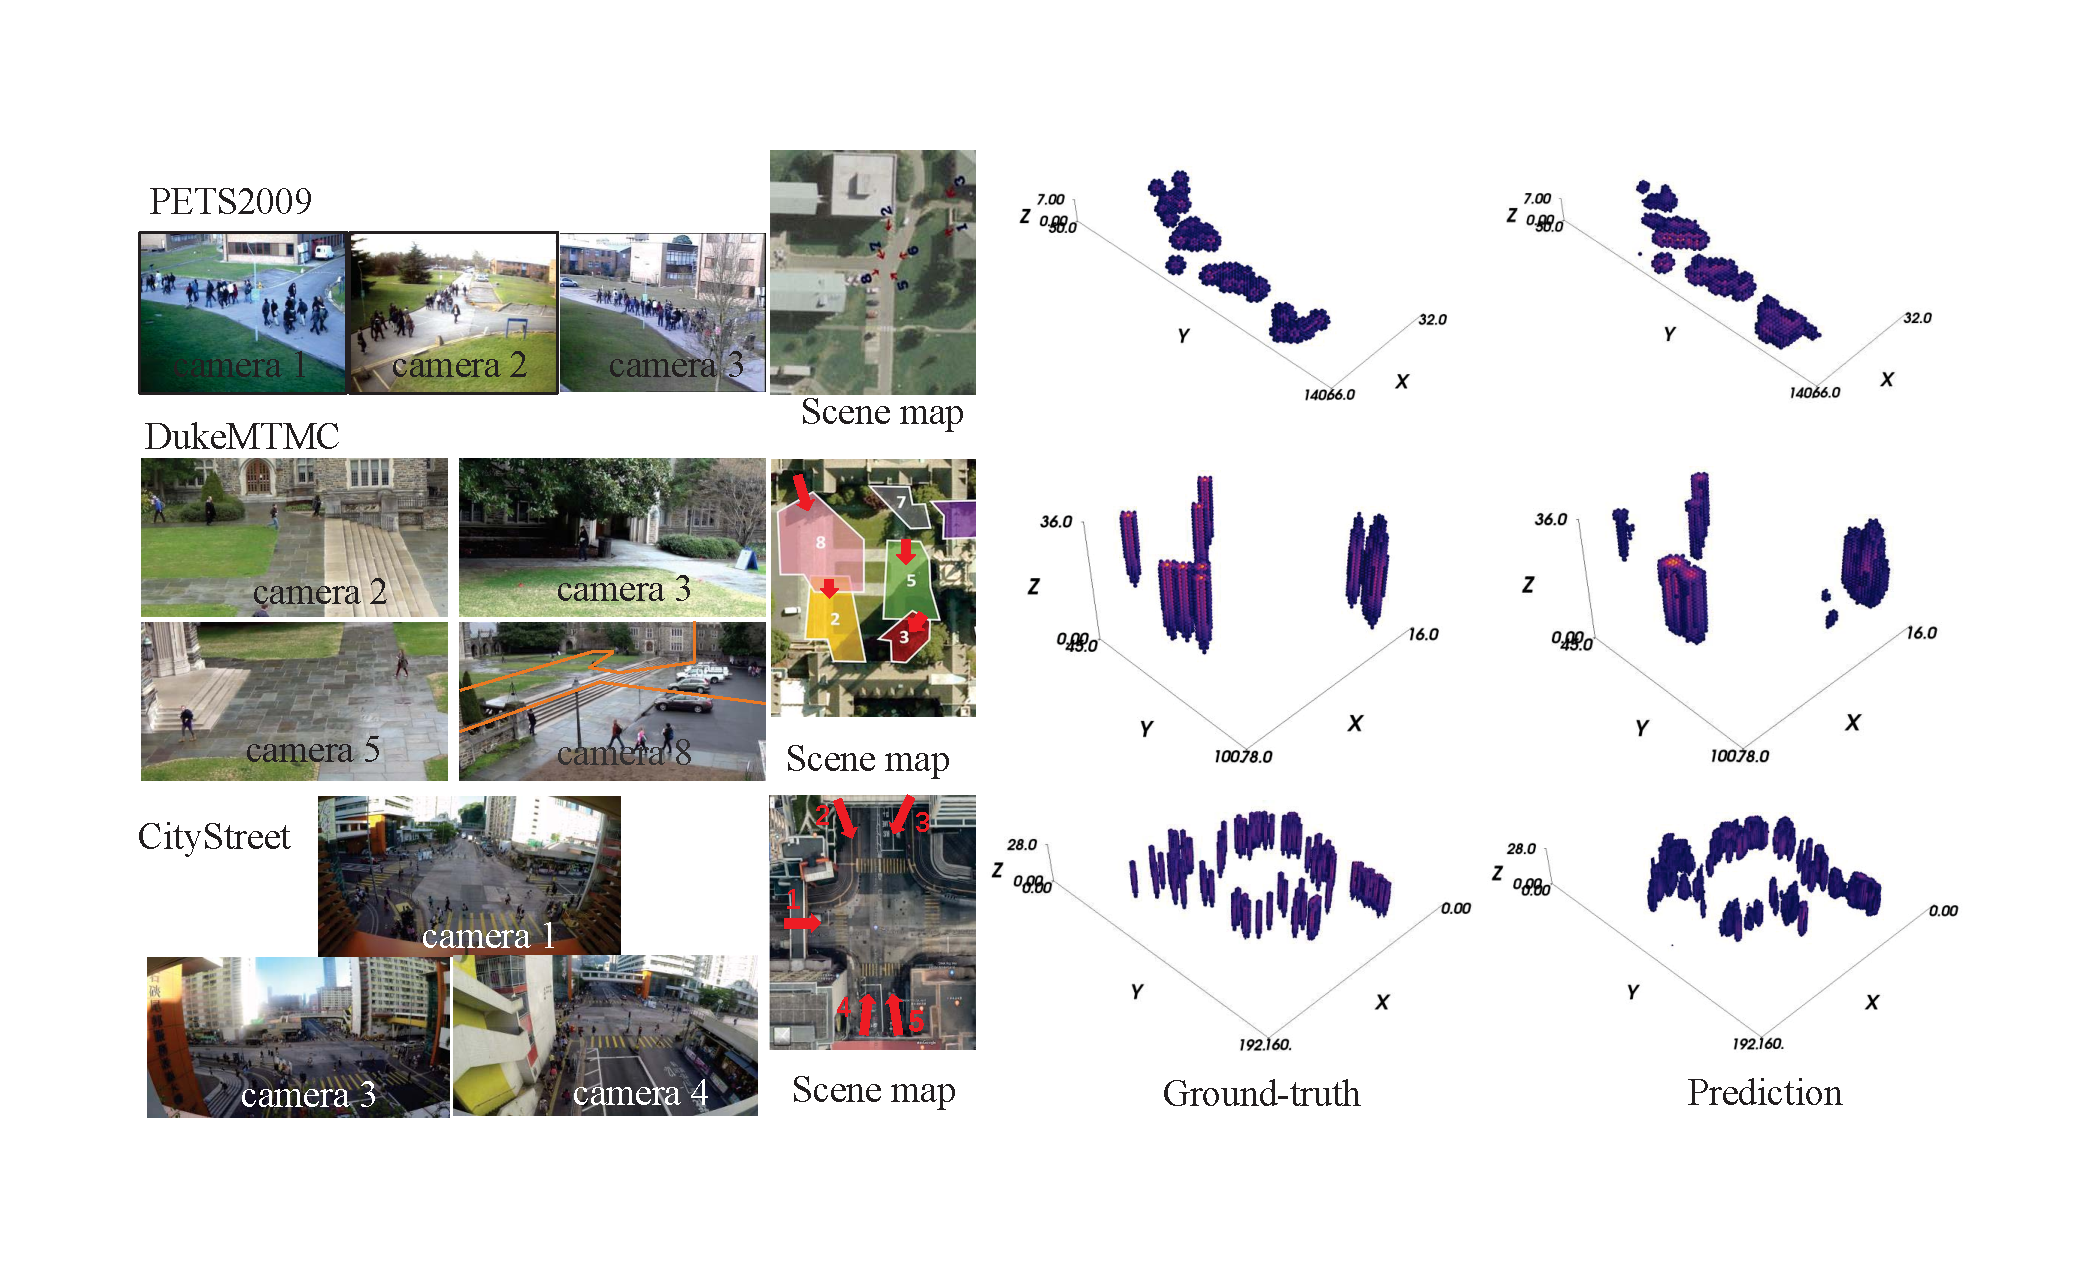
\includegraphics[width=0.85\textwidth]{Fig_results.pdf}
% \end{center}
%%removedVspace
   \caption{Examples of the 3 multi-view datasets and their prediction results.
   %The 3D density maps of PETS2009 are thresholed by 5e-3, while DukeMTMC and CityStreet are thresholded by 1e-3. The 3D ground-truth and predictions are shown from the front, and
   The 3D density maps of PETS2009, DukeMTMC and CityStreet are thresholded by 5e-3, 1e-3 and 1e-3, respectively.
   See the supplemental for more visualizations.}
%   The visualization from top and bottom direction can be found in the Supplemental.}
%%removedVspace
\label{fig:results}
\end{figure*}




\subsection{Experiment results}

The experimental results are shown in Table \ref{table:results} and the visualization results can be found in the Fig. \ref{fig:results} (also see the Supplemental). On \textbf{PETS2009}, the proposed 3D multi-view counting method can achieve better results than the two baseline multi-view counting methods (``Dmap weighted'', ``Detection + ReID'') and the 3 versions of the end-to-end multi-view counting method proposed in \citealp{zhang2019wide}. The first two baseline methods cannot effectively fuse the multi-view information, which limits their performance. The proposed method achieves better performance than MVMS \citep{zhang2019wide}, which shows the advantage of the 3D projection and 3D fusion.
On \textbf{DukeMTMC}, our 3D multi-view counting method achieves comparable performance to the MVMS \citep{zhang2019wide}. But the proposed method still achieves better performance than the two baseline methods. Due to low crowd count and lack of occlusions in the DukeMTMC, the performance gap is not very obvious. On \textbf{CityStreet}, our 3D multi-view counting method achieves the best results among the end-to-end multi-view counting method (late fusion, naive early fusion, MVMS) and the two baseline methods. ``Detection + ReID'' performs badly on CityStreet due to large crowd count and severe occlusions.



\subsection{Ablation study}

In this section, we perform ablation studies on the training loss and the ground-truth settings.

\textbf{Training loss.}
%\textbf{Single-view prediction branch.}
%We compare training with different losses, 3D, 3D+2D and 3D+2D+PCM, in Table \ref{table:ablation_study}.
The rows of Table \ref{table:ablation_study} show the results of using 3D loss, 3D+2D loss or 3D+2D+PCM loss on the 3 datasets. It can be observed using single-view prediction branches and 2D supervision (3D+2D loss) can achieve better multi-view counting performance in comparison with only using 3D loss.
%\textbf{Projection consistency measure.}
Furthermore, using 3D+2D together with PCM loss can obtain better multi-view counting performance compared to using only 3D loss or 3D+2D loss on all 3 datasets with different ground-truth settings.


\textbf{Ground-truth setting.}
The columns of Table \ref{table:ablation_study} show the results of using different resolution of the 3D density map ($n$ is the number of voxels in the $z$-dimension, and $h$ is the voxel height in the 3D world).
% decided by different z-dim voxel number $n$ and voxel height $h$ in the 3D world.
For PETS2009, the best performance is achieved by using voxel number 7 and voxel height 40cm with 3D+2D+PCM loss ($\gamma=100$). For DukeMTMC, using voxel number 36 and voxel height 10cm with 3D+2D+PCM loss ($\gamma=0.5$) gives the best result. As to CityStreet, the best result is obtained by using voxel number 28 and voxel height 10cm with 3D+2D+PCM loss ($\gamma=10$). \zq{Compared to DukeMTMC and CityStreet, the best performance of PETS2009 is achieved at $h$=40cm. The people occlusion in PETS2009 is more severe and many people's lower bodies are totally occluded from all views (e.g., the people in the middle).
%. and we can only observe many people's heads (people in the middle) even with multi-views.
Thus, increasing the height resolution does not provide additional information of the body, but may introduce more noises (other people's features) along the $z$-dim, thus leading to worse performance.}
%making the location identification difficult.
%\NOTE{why is PETS best performance is 40cm?}

%-------------------------------------------------------------------------
\section{Conclusion and Discussion}
\par In this paper, a DNN-based 3D multi-view counting method is proposed, which fuses camera-views to predict the 3D scene-level density map. 3D projection and fusion are used, which can handle the situation when people are not all located at the same height (e.g., %such as people standing in an elevator and on the ground, or
people standing on a staircase),
%where the audience's seats are of varied height),
and provides a chance to solve the scale variation issue in the 3D space without a scale selection operation. The projection consistency measure between the 3D prediction and 2D density map ground-truth is studied and then utilized in the loss function to refine the 3D prediction further.
Compared to other state-of-art multi-view counting methods, the proposed method  achieves better or comparable counting performance as well as a more informative scene-level crowd representation.


In addition to counting humans, the proposed 3D multi-view counting method can also be applied to counting birds in the sky or the fish in the aquarium, where both the bird or the fish count can be obtained as well as their 3D location distributions -- of course, this requires collecting more multi-view scenes. Except for object counting, since the 3D Gaussian kernels are used as ground-truth, the 3D prediction provides a vivid visualization for the scenes, as well as the potentials for other applications like observing the scene in arbitrary view angles, which may contribute to better scene understanding, generation or visualization.


\section{Acknowledgements}
This work was supported by grants from the Research Grants Council of the Hong Kong Special Administrative Region, China (Project No. [T32-101/15-R] and CityU 11212518).

{\small
\bibliographystyle{aaai}
Suscipit incidunt nemo neque soluta repudiandae quos animi aperiam pariatur nisi, debitis provident ratione voluptates necessitatibus tenetur vitae beatae facere recusandae inventore?Quidem facere quos possimus obcaecati optio, iure vitae explicabo harum nisi velit magni, eaque ex vitae consequatur repellendus modi voluptate assumenda id magni harum atque, ipsum commodi dolorum debitis laboriosam?Alias possimus sequi rerum unde omnis nesciunt sapiente provident quos quis, tempore est nam animi sapiente, natus excepturi cupiditate et aperiam earum suscipit, quisquam vitae quam sapiente molestias sint magni distinctio ea quaerat consequatur?Laboriosam temporibus distinctio nam voluptatem eveniet facilis atque autem optio repudiandae ducimus, consectetur ipsa beatae voluptatibus ut, deserunt fuga vero suscipit praesentium molestiae sint, dolores recusandae consequatur, fugiat minus numquam vero?Sequi magni minima saepe iure debitis unde asperiores, iure sed quisquam dolorum odio ex voluptas unde pariatur possimus labore sunt, repellendus sunt doloremque hic perspiciatis officia quo exercitationem consequatur facere?Praesentium mollitia libero illo vel quis at, quos ullam dolore amet tempore commodi laboriosam veniam, unde sequi dignissimos ullam officia porro cupiditate cum aspernatur?Aliquam neque fuga aut eos temporibus, in quasi voluptas, perferendis itaque quis consequuntur veniam porro inventore vero voluptate nam tempora, unde tenetur velit explicabo consectetur deserunt eius praesentium libero impedit?Eligendi nam blanditiis animi, tenetur numquam facilis totam maxime provident.Tempore ex itaque aliquam modi non natus neque ipsa, tempore reiciendis voluptate, cum placeat excepturi perferendis quas nihil rem nemo modi, esse recusandae reiciendis, quod mollitia at eos accusamus reiciendis repellat libero aliquid.\clearpage
\bibliography{egbib}
}

\end{document}